\documentclass[12pt]{extarticle}
\usepackage[utf8]{inputenc}
\usepackage{mathtools} % matrices, cases
\usepackage{amsfonts} % natural/whole/real/etc. number sets
\usepackage{geometry}
\usepackage{graphicx}
\geometry{verbose,a4paper,tmargin=0.8cm,bmargin=0.8cm,lmargin=0.8cm,rmargin=0.8cm}
\setlength{\parindent}{0cm}

\begin{document}
	% \huge \underline{} \\
	{\large
		Carti: \\
		Limbaje formale si automate - A. Atanasiu \\
		Introduction to Automata theory, languages and computation. - J. Hopcroft, J. Ullman \\
		\\
		$\Sigma_{1} = \{ 0, 1 \}$ \\
		$\Sigma_{2} = \{ 0, 1, ..., 9 \}$ \\
		$\Sigma_{3} = \{ a, b, ..., Z \}$ \\
		\\
		$a \cdot b = ab \neq ba$ \\
		$a \cdot \lambda = \lambda \cdot a = a$ \\
		$\alpha \cdot \lambda = \lambda \cdot \alpha = \alpha$ \\
		\\
		$A \cdot B = \{ a_{i}, b_{j} / a_{i} \in A, b_{j} \in B \}$ \\
		$A^{0} = \{ \lambda \}$ \\
		$A^{k+1} = A^{k} \cdot A$ \\
		$\Sigma_{1}^{2} = \Sigma_{1} \cdot \Sigma_{1} = \{ 00, 01, 10, 11 \}$ \\
		$A' = A$ \\
		$\Sigma_{1}^{3} = \Sigma_{1}^{2} \cdot \Sigma_{1} = \{ 000, 001, 010, ..., 111 \}$ \\
		$\Sigma_{1}^{k} = \{ a_{1}, ..., a_{k} / a_{i} \in \Sigma_{1} \}$ \\
		$A^{*} = \underset{k \geq 0}{\bigcup}A^{k} = A^{0} \cup A^{1} \cup ...$ \\
		$\Sigma_{1}^{*} = \{ \alpha / \exists k \in \mathbb{N}, \alpha = a_{1}, ..., a_{k}, a_{i} \in \Sigma_{1} \}$
		$\Sigma_{2}^{*} =$ toate numerele \\
		\\
		Problema capra varza lup: \\
		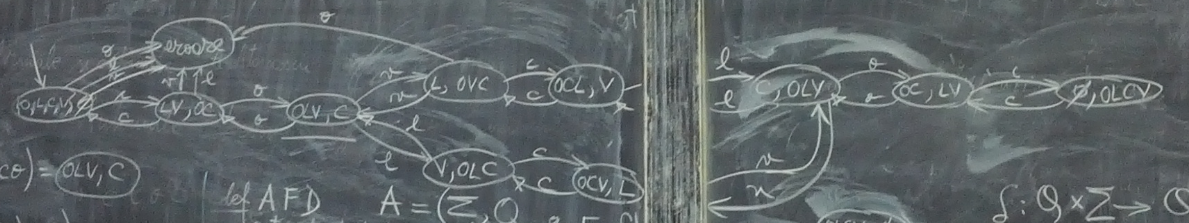
\includegraphics[width=\textwidth]{figura1.png} \\
		\underline{def.} Automat Finit Determinist (AFD): $A = (\Sigma, Q, q_{0}, F, \delta)$ \\
		$\Sigma$ = alfabet (finit) \\
		$Q$ = multimea de stari (finită) \\
		$q_{0}$ = starea initială \\
		$F$ = starea finală \\
		$\delta : Q \times \Sigma \rightarrow Q$ = functia de tranzitie \\
		$\delta \rightarrow \quad \overset{\sim}{\delta} : Q \times \Sigma^{*} \rightarrow Q $ \\
		$\overset{\sim}{\delta}(q, \lambda) = q$ \\
		$\overset{\sim}{\delta}(q, a \cdot \alpha) = \delta (\underset{q_{1}}{\underbrace{\delta(q, \lambda)}}, \alpha)$ \\
		$\overset{\sim}{\delta}(q, \lambda) = \overset{\sim}{\delta}(\underset{q'}{\underbrace{\delta(q, \lambda)}}, \lambda) = \delta\underset{q'}{\underbrace{(q, a)}}$ \\
		\\
		\underline{def.} $L(A) = \{ \alpha \in \Sigma^{*} / \widetilde{\delta}(q_{0}, \alpha) \in F \}$ \\
		$L(A) = \{ covcloc, cccovclooo, ... \}$ \\
		$L(A) = \{ a^{n} / n \geq 0 \} = \{ \alpha, a, aa, aaa, ... \}$ \\
		$A = (\Sigma, Q, q_{0}, F, \delta)$ \\
		$\underset{(AFD)}{\underline{Obs.}} \lambda \in L(A) \Leftrightarrow \widetilde{\delta}\underset{\underset{q_{0}}{\parallel}}{(q_{0}, \lambda)} \in F \Leftrightarrow q_{0} \in F$ \\
		$\lambda \notin L(A) \Leftrightarrow q_{0} \notin F$ \\
		$L(A) = \{ a^{n} / n \geq 1 \} = \{ a, a^{2}, a^{3}, ... \}$ \\
		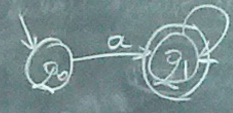
\includegraphics[width=5cm]{figura2.png} \\
		\\
		$L(A) = \{ a, b \}^{*} = \{ \alpha, a, b, ab, ba, aab, bab, ... \}$ \\
		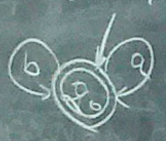
\includegraphics[width=3.5cm]{figura3.png} \\
		\\
		$L(A) = \{ a^{n} \cdot b^{m} / m, n \geq 0 \} = \{ \alpha, a, b, ab, a^{2}b, ab^{2}, ... \}$ \\
		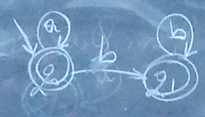
\includegraphics[width=5cm]{figura4.png} \\
		\begin{tabular}{ l | l | l }
			$\delta$ & a & b \\ \hline
			$q_{0}$ & $q_{0}$ & $q_{1}$ \\ \hline
			$q_{1}$ & $\emptyset$ & $q_{1}$ \\
		\end{tabular} \\
		\\
		$L(A) = \{ a^{n} \cdot b^{m} / m, n \geq 1 \}$ \\
		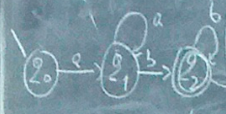
\includegraphics[width=5cm]{figura5.png} \\
		\\
		$L(A) = \{ a^{2k + 1} / k \geq 0 \} = \{ a, a^{3}, a^{5}, a^{7}, a^{9}, ... \}$ \\
		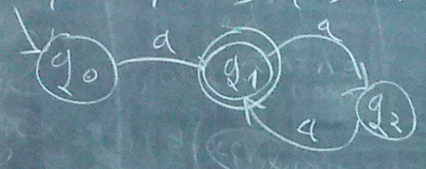
\includegraphics[width=5cm]{figura6.png} \\
		\\
		$L(A) = \{ \alpha a a \beta / \alpha, \beta \in \{ a, b \}^{*} \} = \{ aa, baa, aab, aaa, ababaaabab, ... \}$ \\
		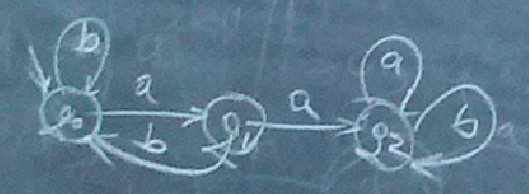
\includegraphics[width=5cm]{figura7.png} \\
		\\
		$L(A) = \{ \alpha a \beta a \gamma / \alpha, \beta, \gamma \in \{ a, b \}^{*} \}$ \\
		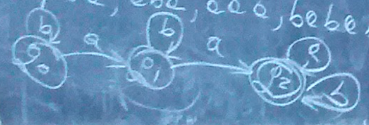
\includegraphics[width=5cm]{figura8.png} \\
		\\
		Temă: $L(A) = \{ \alpha \in \{ a, b \}^{*} / $ nr. par de a, nr. par de b $\}$
	}
\end{document}